\pdfmapfile{+univers}%
\pdfmapfile{+dinbold}%
\documentclass[ngerman]{beamer}
\usepackage[utf8]{inputenc}
\usepackage[T1]{fontenc}
\usepackage[ngerman]{babel}
\usepackage{graphicx}
\usepackage{svg}
\usetheme[pagenum,nosectionnum,noheader,transition=push,headline=light]{tud}
\begin{document}
\title{FoodShip Final Presentation}
\subtitle{FoodShip, a foodsharing App}
\author{Sönke Huster \& Hannes Hilbert}
\date{\today}

\maketitle

%  \frame{\frametitle{Inhaltsverzeichnis}\tableofcontents}
\section{Foodship}
\section{First Startup and Offline Challenge}
\frame{\frametitle{Login / Registration}
	\begin{itemize}
		\item User enters Name and Location
		\item \textbf{Offline Challenge:} API-Calls are always cached and sent when server is reachable
	\end{itemize}
	\begin{figure}
		\begin{center}
			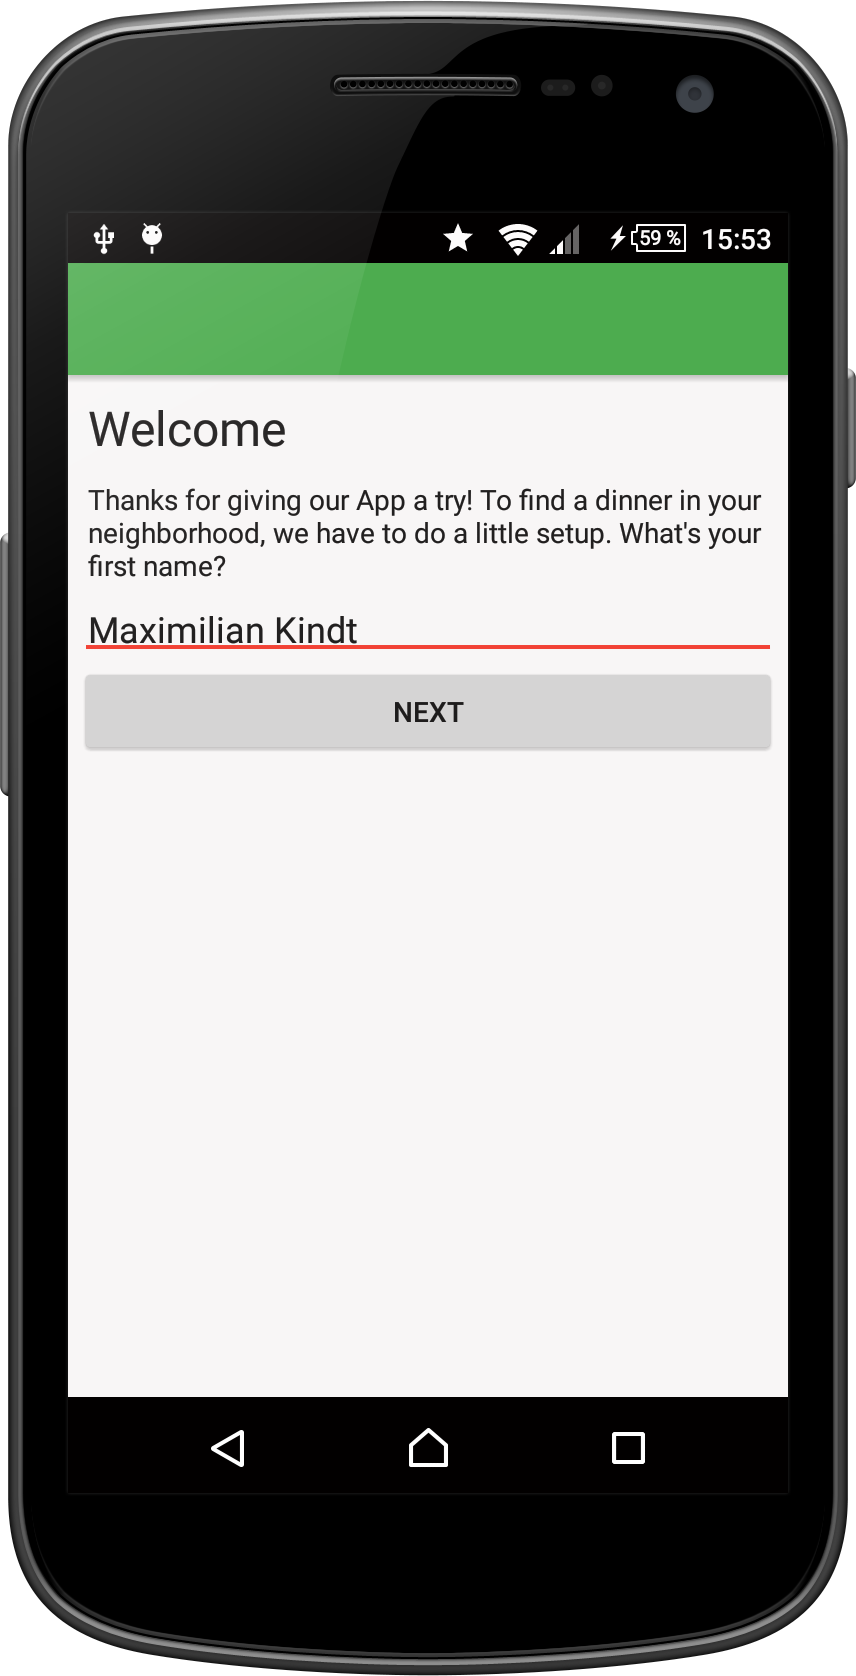
\includegraphics[width=0.25\textwidth,height=\textheight,keepaspectratio]{screenshots/1_enter_name.png}
			\hspace{1cm}
			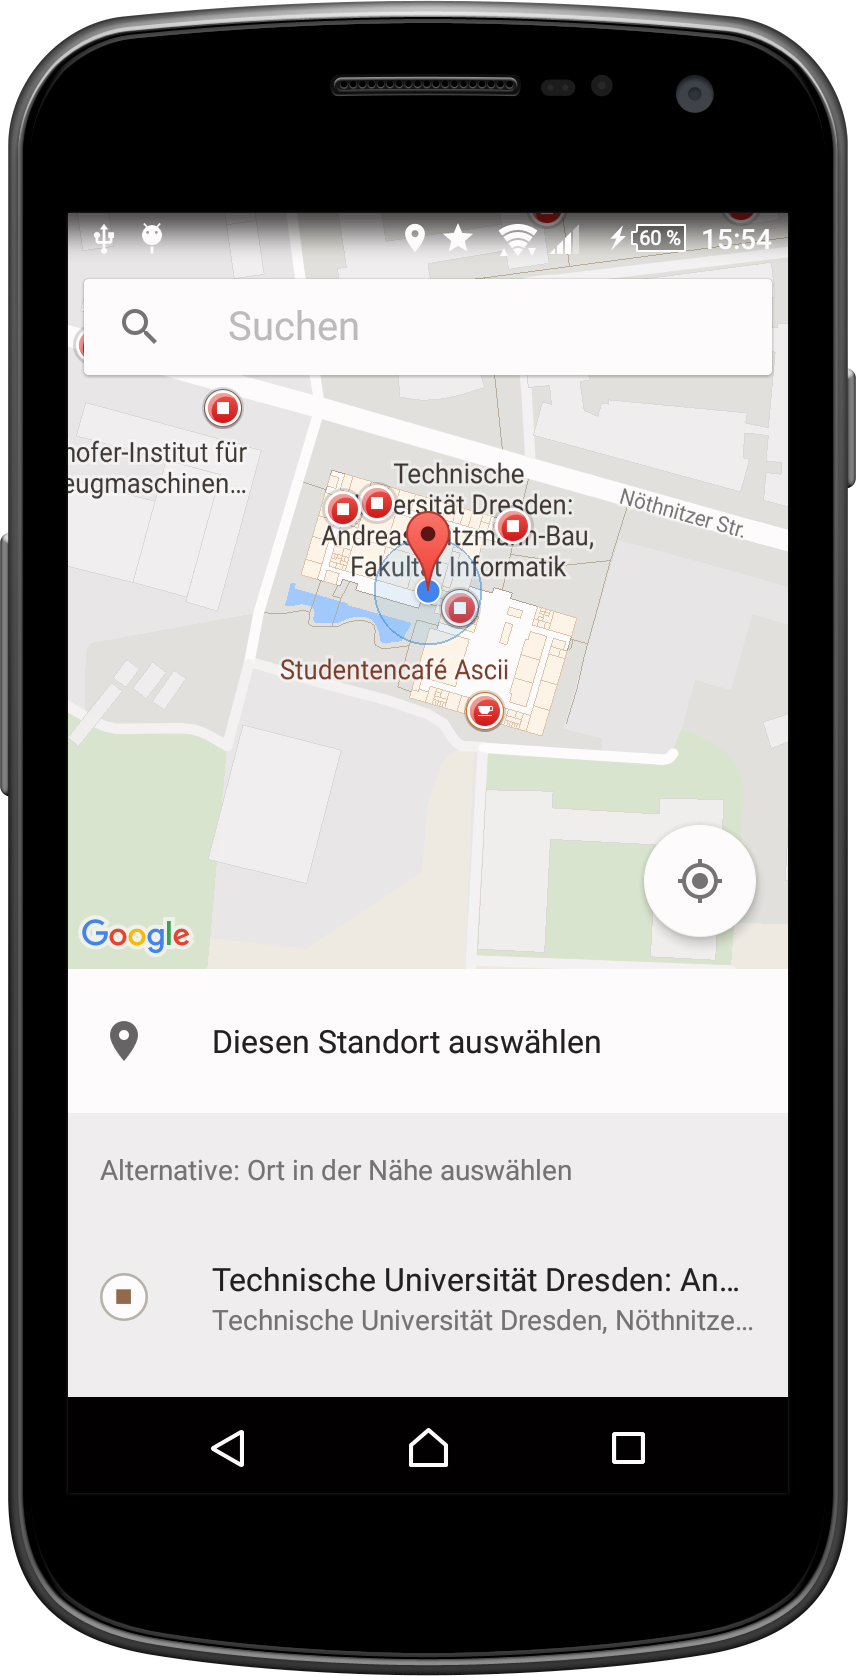
\includegraphics[width=0.25\textwidth,height=\textheight,keepaspectratio]{screenshots/2_enter_location.png}
		\end{center}
	\end{figure}
}
\section{MainScreen and Ingredience Adaptation}
\frame{\frametitle{Digital Pantry}
	\begin{itemize}
		\item Products are added to digital personal pantry
		\item API Feedback is emulated, when server is not reachable
	\end{itemize}
	\begin{figure}
		\begin{center}
			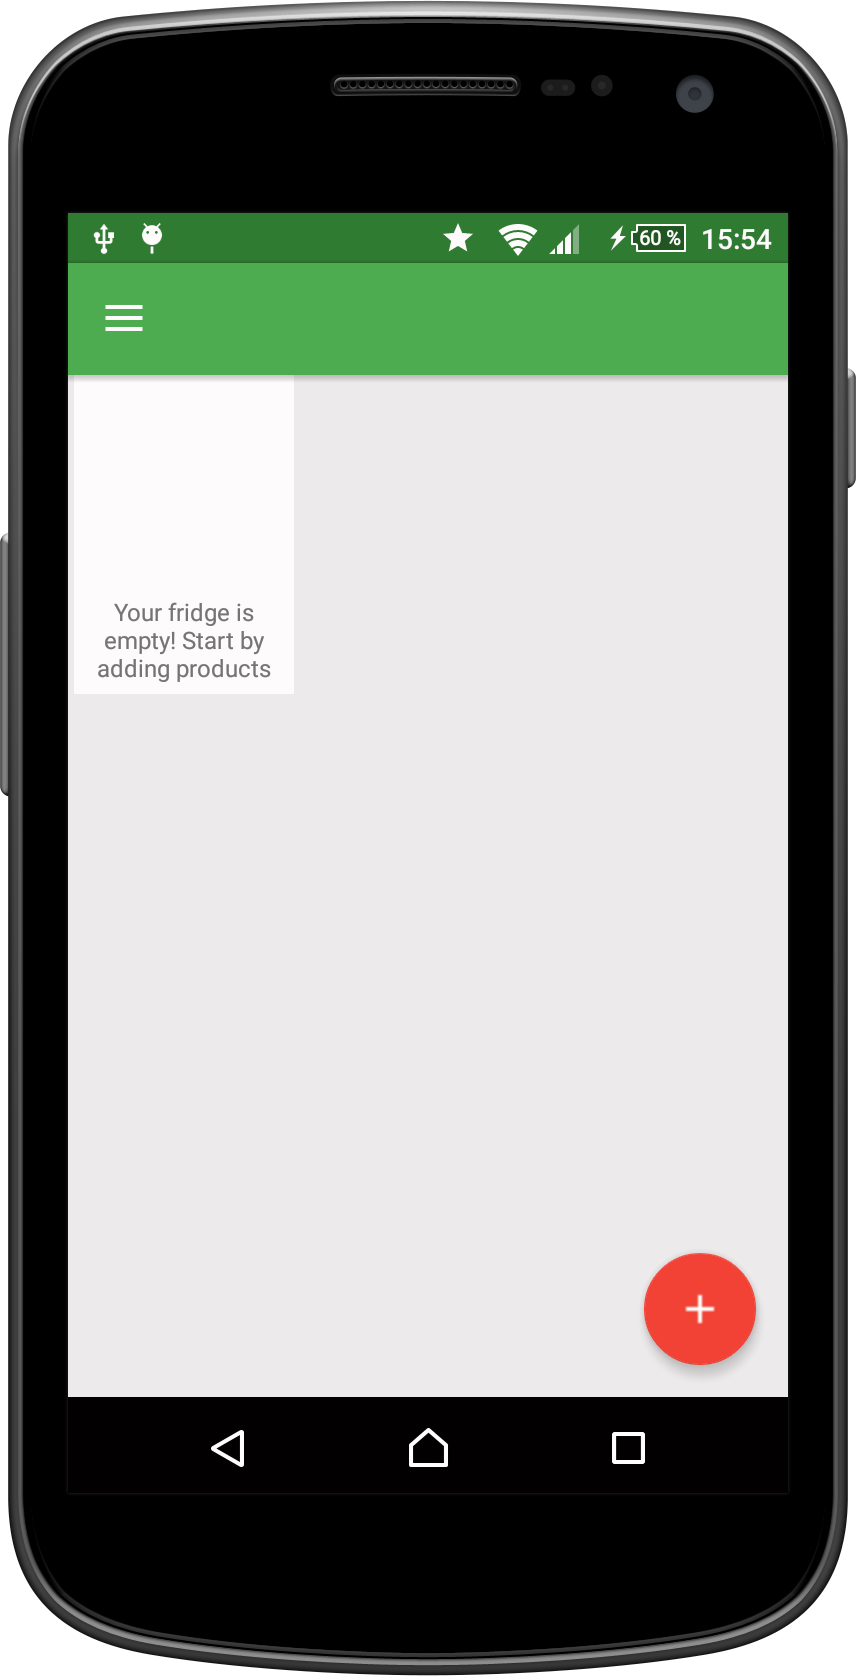
\includegraphics[width=0.25\textwidth,height=\textheight,keepaspectratio]{screenshots/3_empty_fridge.png}
			\hspace{1cm}
			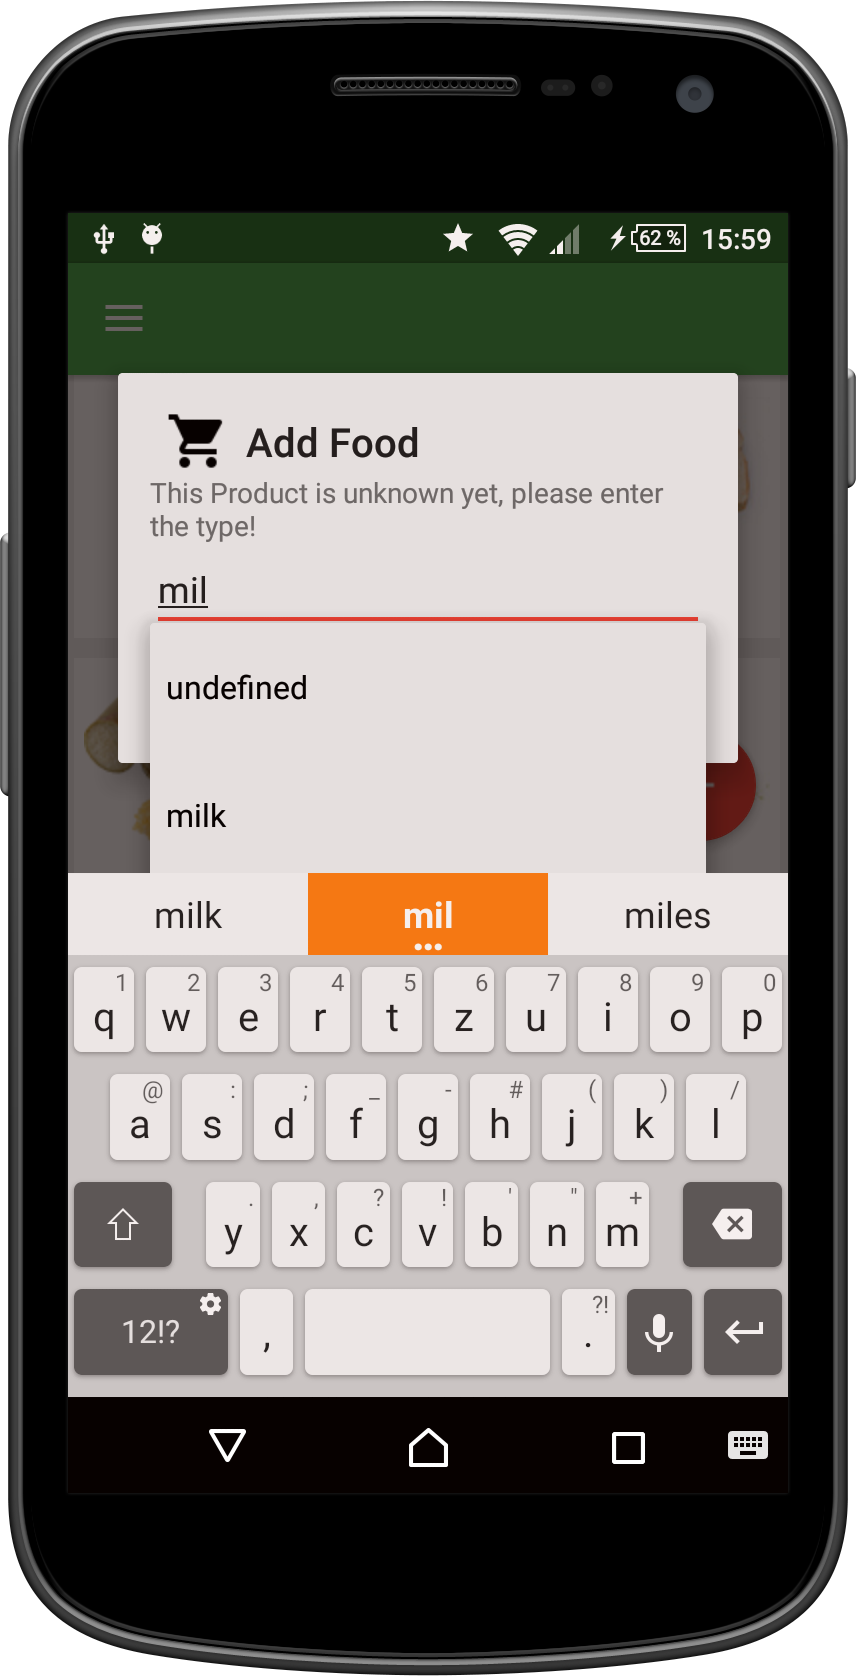
\includegraphics[width=0.25\textwidth,height=\textheight,keepaspectratio]{screenshots/5_add_to_fridge.png}
			\hspace{1cm}
			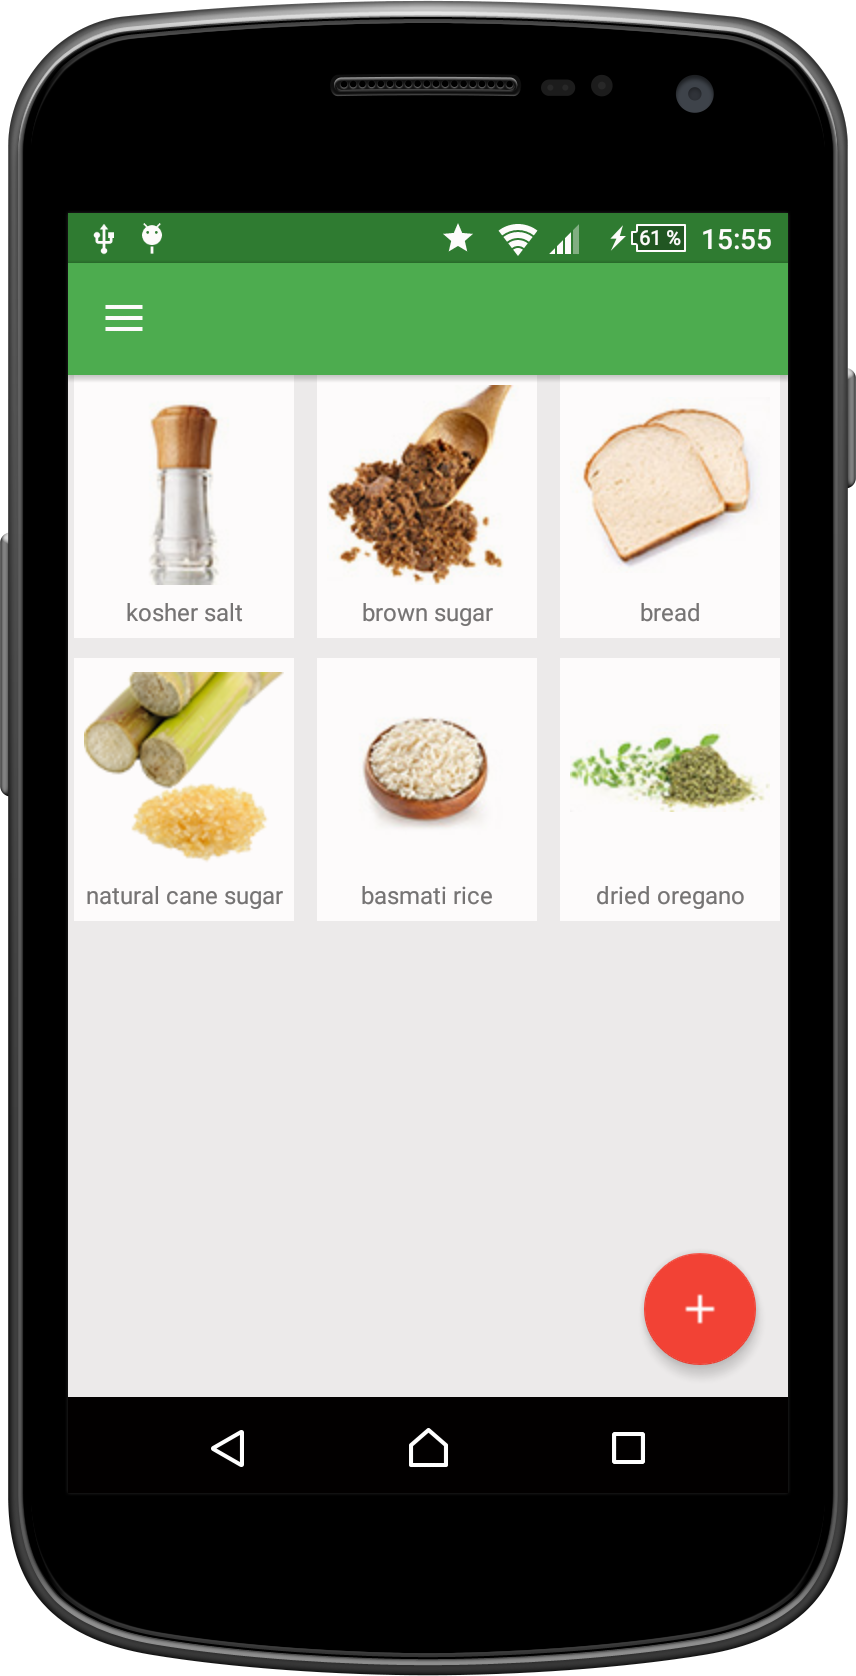
\includegraphics[width=0.25\textwidth,height=\textheight,keepaspectratio]{screenshots/4_full_fridge.png}
		\end{center}
	\end{figure}
}



\section{Notification and Prefetching}
\frame{\frametitle{Notification \& Group View}
	\begin{itemize}
		\item Daily notification is sent to users in the same area
		\item User can accept or deny invitation
		\item User can vote recipes
	\end{itemize}
	\begin{figure}
		\begin{center}
			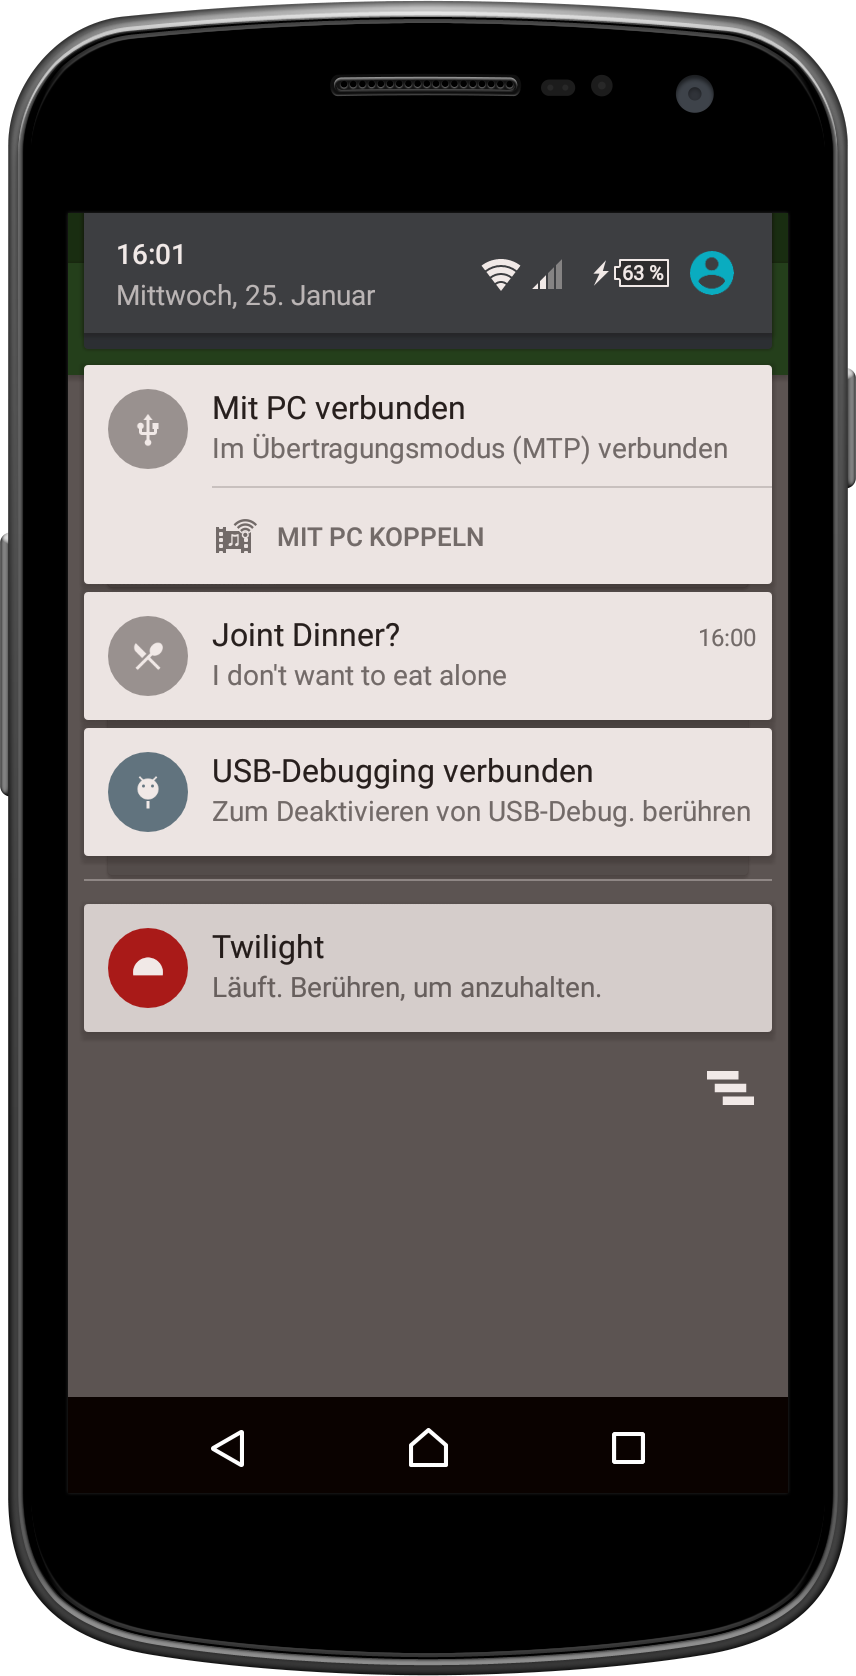
\includegraphics[width=0.25\textwidth,height=\textheight,keepaspectratio]{screenshots/6_notification.png}
			\hspace{1cm}
			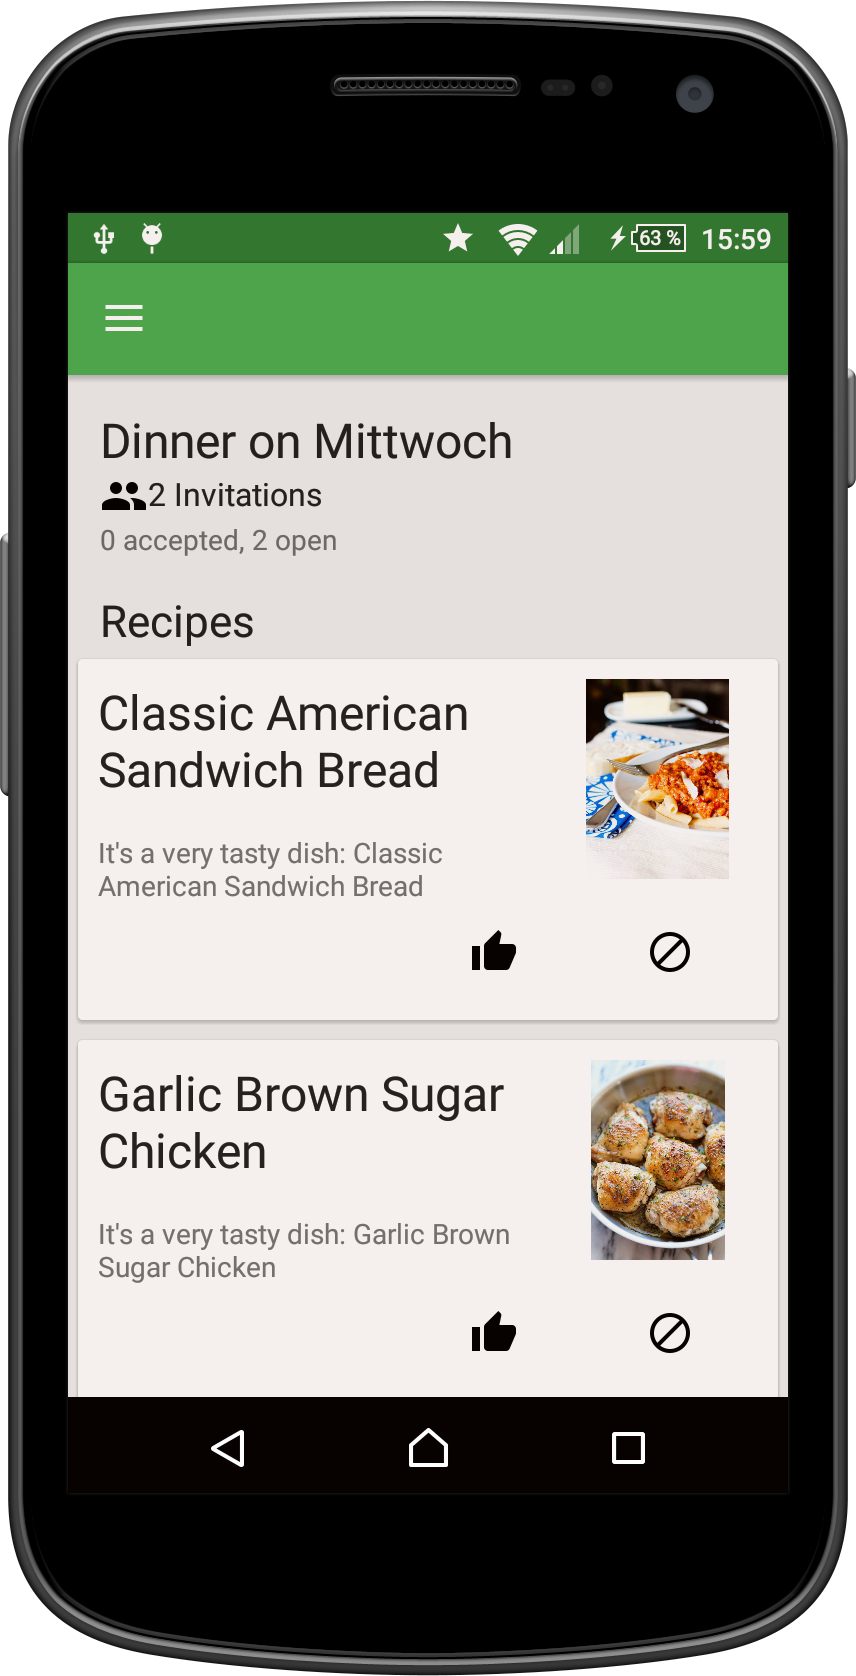
\includegraphics[width=0.25\textwidth,height=\textheight,keepaspectratio]{screenshots/7_recipe_view.png}
		\end{center}
	\end{figure}
}

\section{Adaptation Concepts}
\frame{\frametitle{Other Adaptation Concepts}
	\begin{itemize}
		\item Location-Context: Find groups of people nearby
		\item Prefetching: App prefetches group information and recipe pictures after notification
		\item Ingredients as Context: Suggests recipes, that match a maximum of ingredients
		\item Data is persisted in internal storage and in cache for better user experience
	\end{itemize}
	\begin{figure}
		\begin{center}
			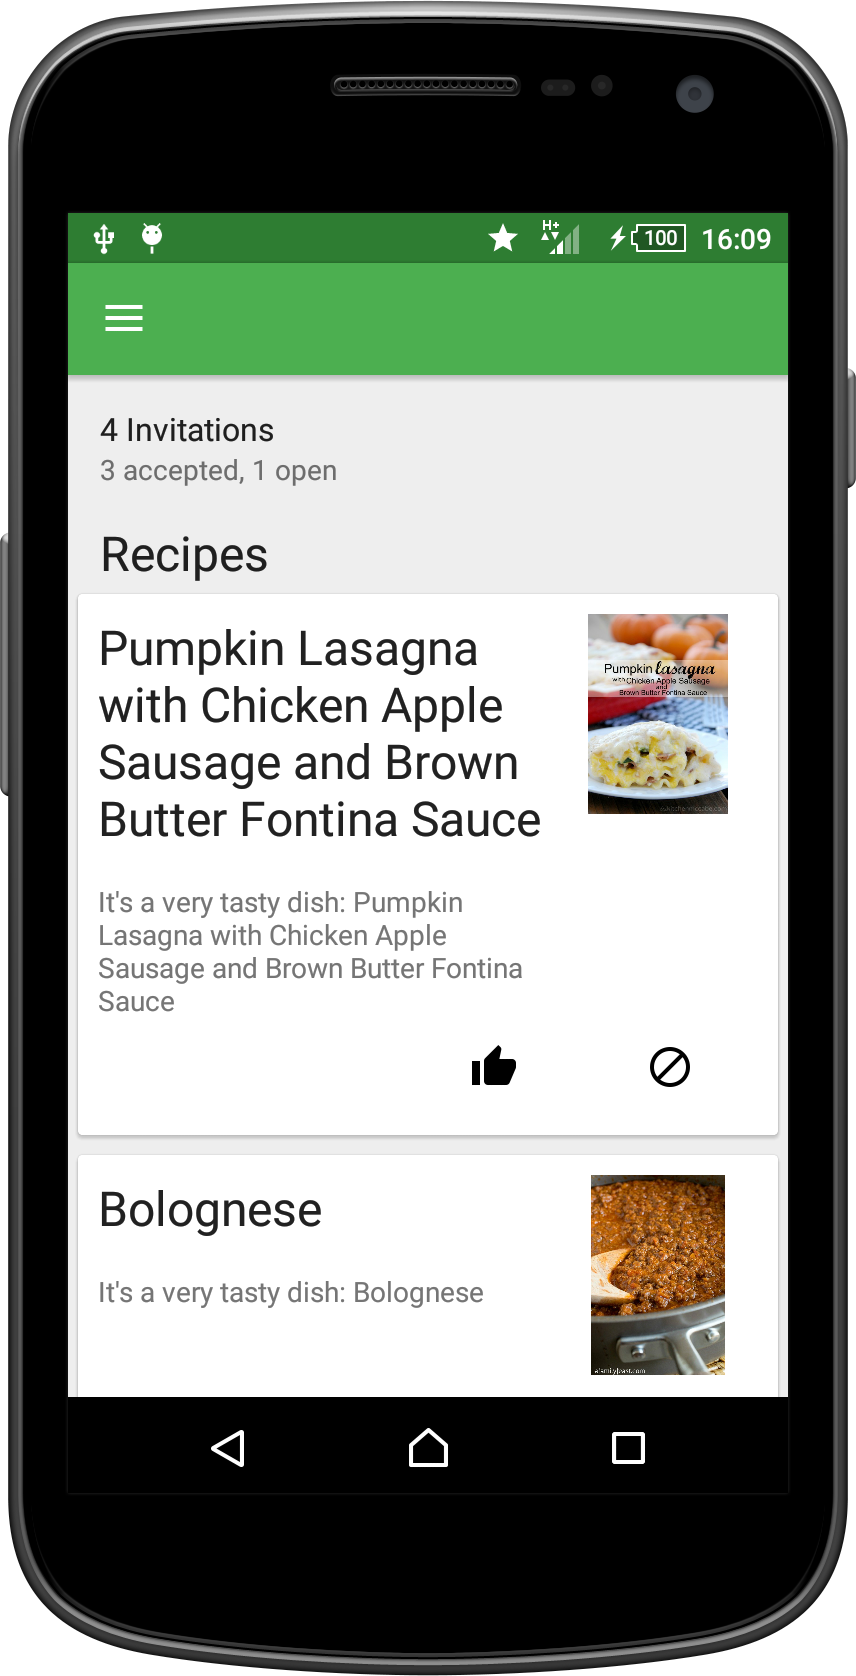
\includegraphics[width=0.2\textwidth,height=\textheight,keepaspectratio]{../screenshots/recipe_overview.png}
			\hspace{1cm}
			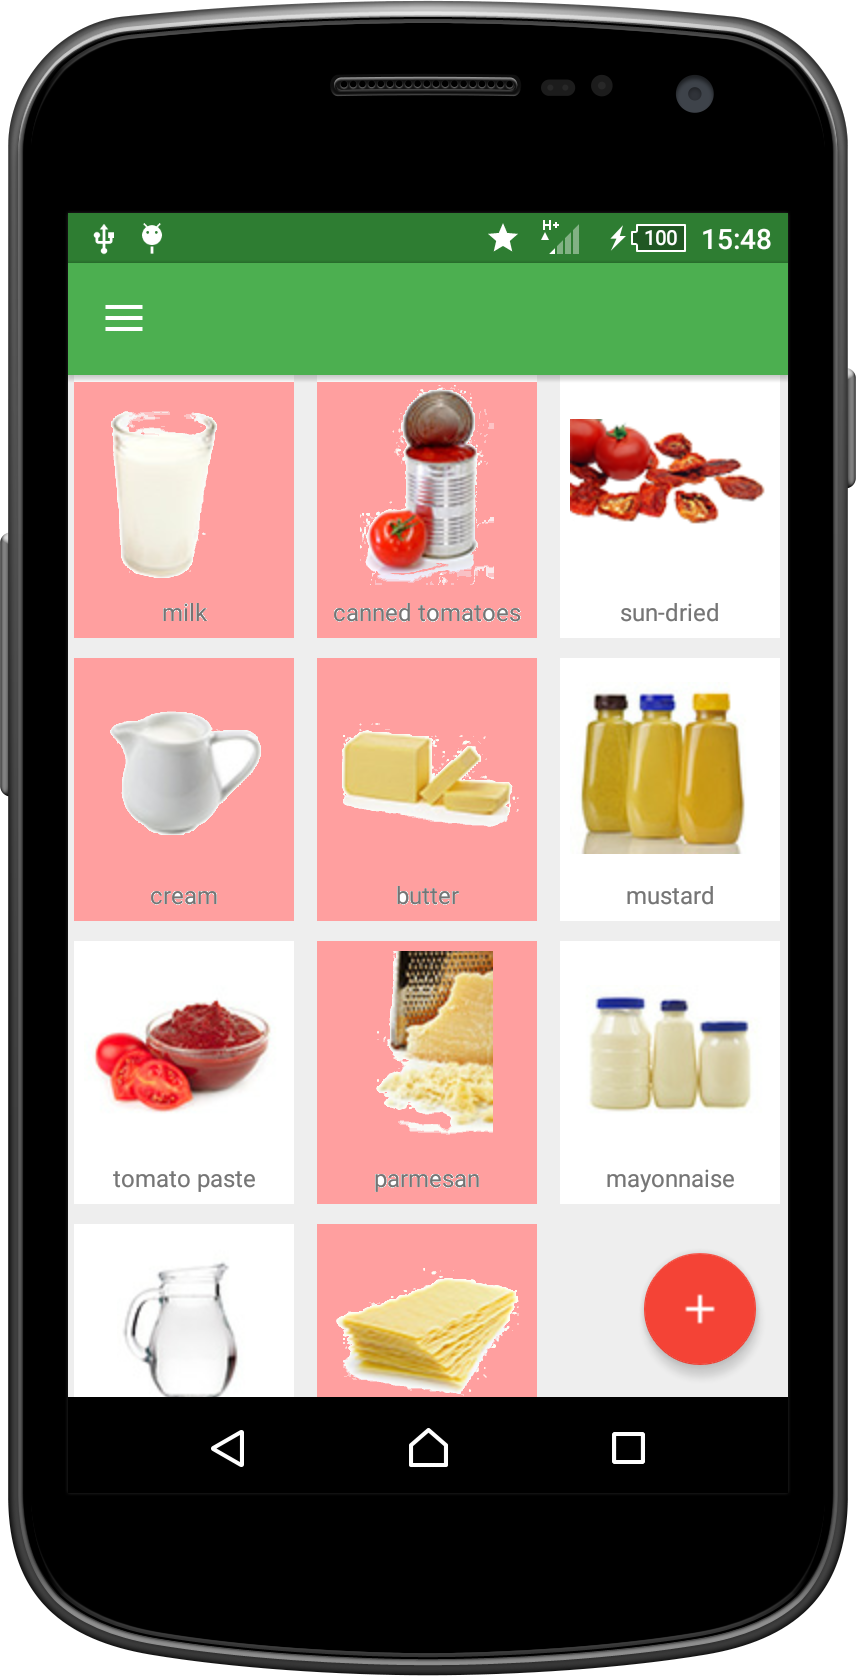
\includegraphics[width=0.2\textwidth,height=\textheight,keepaspectratio]{../screenshots/recipe_ingredients.png}
		\end{center}
	\end{figure}
}

\section{Architecture}
\frame{\frametitle{Architecture \& Technologies}
	\begin{figure}
		\centering
		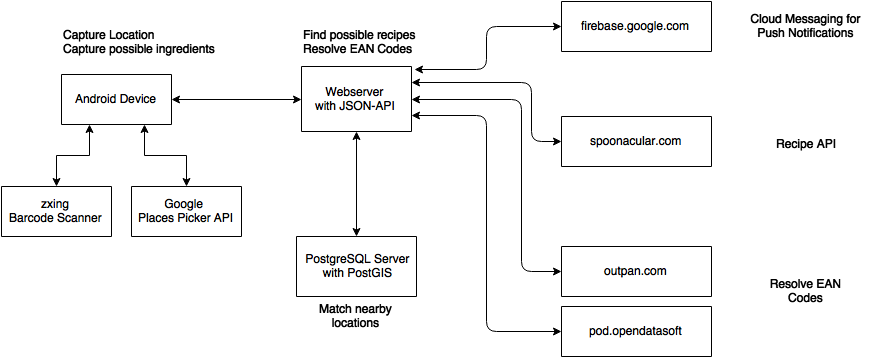
\includegraphics[width=0.9\textwidth,height=\textheight,keepaspectratio]{../diagrams/architecture_2.png}
	\end{figure}
}


\end{document}
